\section{Text Access}

\subsection{Two Modes of Text Access: Pull vs. Push}
\begin{itemize}
\item Pull Mode (search engines) – Users take initiative
    \begin{itemize}
    \item Ad hoc information need
    \end{itemize}
\item Push Mode (recommender systems)
    \begin{itemize}
    \item Systems take initiative
    \item Stable information need or system has good knowledge about a user’s need
    \end{itemize}
\end{itemize}


\begin{figure}[H]
    \centering
    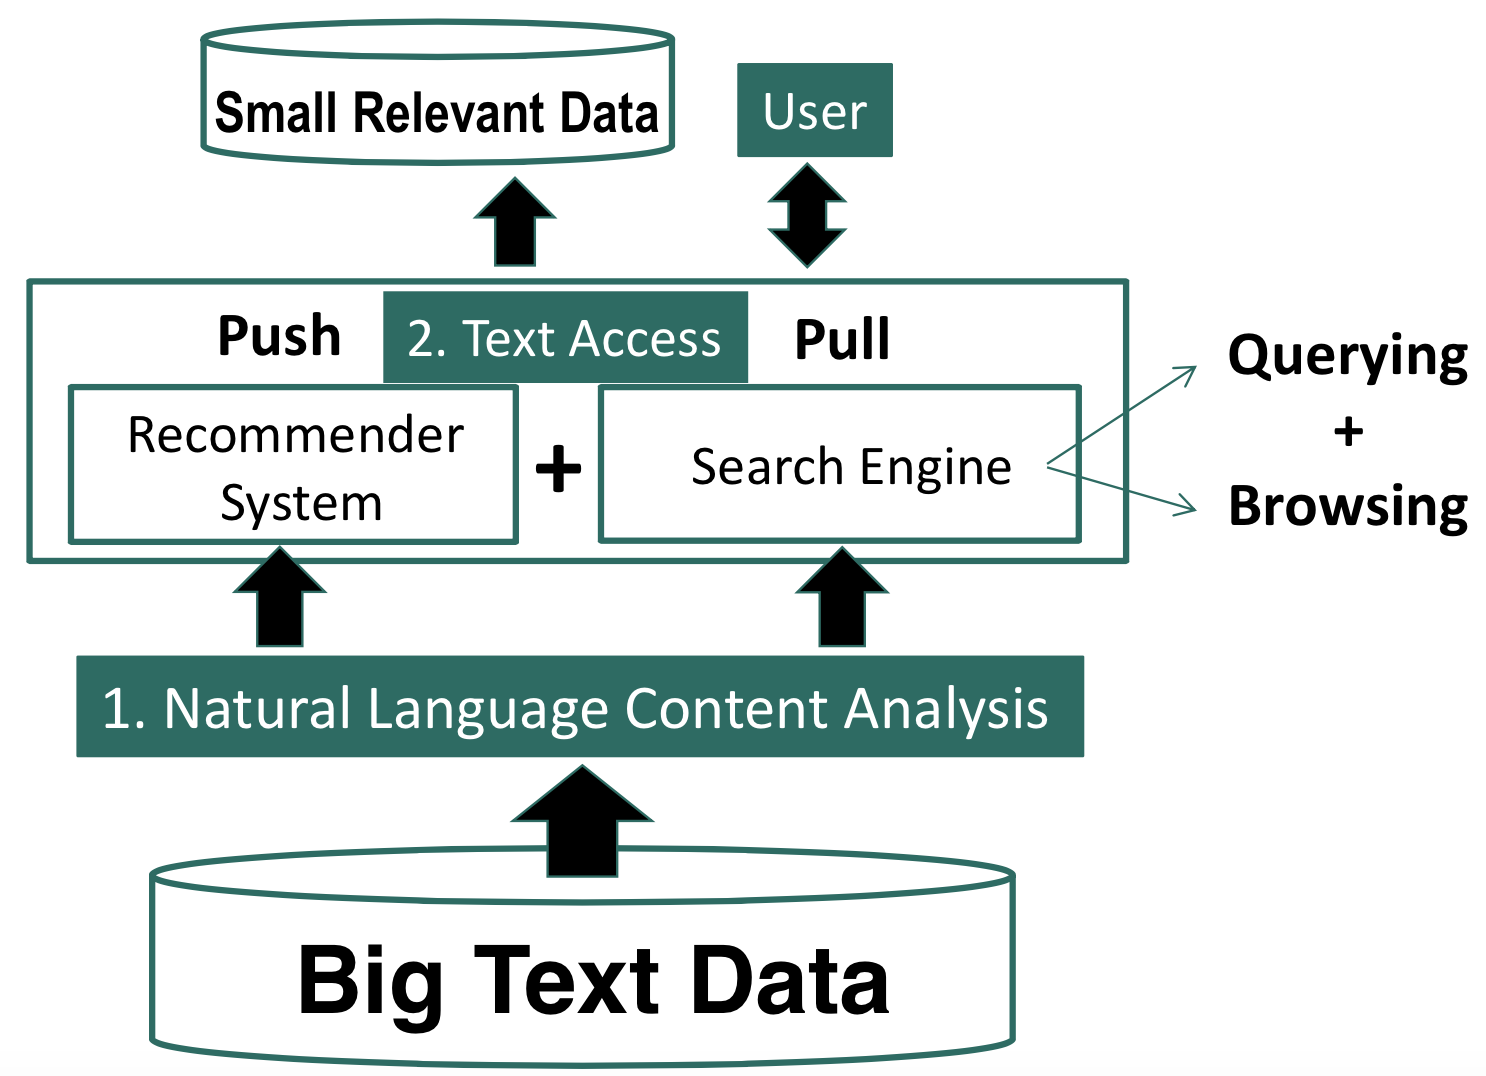
\includegraphics[width=0.6\linewidth]{text_access.png}
\end{figure}


\subsection{Pull Mode: Querying vs. Browsing}
\begin{itemize}
\item Querying
    \begin{itemize}
    \item User enters a (keyword) query
    \item System returns relevant documents
    \item Works well when the user knows what keywords to use
    \end{itemize}
\item Browsing
    \begin{itemize}
    \item User navigates into relevant information by following a path
enabled by the structures on the documents
    \item Works well when the user wants to explore information, doesn’t know what keywords to use, or can’t conveniently enter a query
    \end{itemize}
\end{itemize}


\subsection{Recommended reading}
\begin{itemize}
\item N. J. Belkin and W. B. Croft. 1992. <<Information filtering and information retrieval: two sides of the same coin?>> Commun. ACM 35, 12 (Dec. 1992), 29-38.
\end{itemize}